\PassOptionsToPackage{unicode=true}{hyperref} 
\PassOptionsToPackage{hyphens}{url}

\documentclass[]{article}

% Package section
\usepackage{lmodern}
\usepackage{amssymb,amsmath}
\usepackage{ifxetex,ifluatex}
% packages for tables
\usepackage{array}
\usepackage[longtable]{multirow}
\usepackage{ragged2e}
\usepackage{longtable}
\usepackage{graphicx}
\usepackage{colortbl}
\usepackage{graphicx}
\usepackage[section]{placeins}
\graphicspath{ {./images/} }

% \usepackage[margin=1.5in]{geometry}
\usepackage[a4paper, total={6in, 8in}]{geometry}

\usepackage{titlesec}
\titlespacing{\section}{0pt}{*6}{*3}
\titlespacing{\subsection}{0pt}{*4}{*2}
\titlespacing{\subsubsection}{0pt}{*4}{*2}
\titlespacing{\paragraph}{0pt}{*3}{*2}


\usepackage{enumitem}
\usepackage{fixltx2e} % provides \textsubscript
\ifnum 0\ifxetex 1\fi\ifluatex 1\fi=0 % if pdftex
  \usepackage[T1]{fontenc}
  \usepackage[utf8]{inputenc}
  \usepackage{textcomp} % provides euro and other symbols
\else % if luatex or xelatex
  \usepackage{unicode-math}
  \defaultfontfeatures{Ligatures=TeX,Scale=MatchLowercase}
\fi
% use upquote if available, for straight quotes in verbatim environments
\IfFileExists{upquote.sty}{\usepackage{upquote}}{}
% use microtype if available
\IfFileExists{microtype.sty}{%
\usepackage[]{microtype}
\UseMicrotypeSet[protrusion]{basicmath} % disable protrusion for tt fonts
}{}
\IfFileExists{parskip.sty}{%
\usepackage{parskip}
}{% else
\setlength{\parindent}{0pt}
\setlength{\parskip}{6pt plus 2pt minus 1pt}
}

\usepackage{hyperref}
\hypersetup{
        colorlinks=true,
        urlcolor=blue,
        linkcolor=blue
}
\urlstyle{same}  % don't use monospace font for urls

\setlength{\emergencystretch}{3em}  % prevent overfull lines
\providecommand{\tightlist}{%
  \setlength{\itemsep}{0pt}\setlength{\parskip}{0pt}}
\setcounter{secnumdepth}{0}
% Redefines (sub)paragraphs to behave more like sections
\ifx\paragraph\undefined\else
\let\oldparagraph\paragraph
\renewcommand{\paragraph}[1]{\oldparagraph{#1}\mbox{}}
\fi
\ifx\subparagraph\undefined\else
\let\oldsubparagraph\subparagraph
\renewcommand{\subparagraph}[1]{\oldsubparagraph{#1}\mbox{}}
\fi

% set default figure placement to htbp
\makeatletter
\def\fps@figure{htbp}
%\makeatother

%-------------------------------------------------------------------------------------%

\title{Cross-Media Measurement System for Reach and Frequency}
\author{WFA Cross-Media Measurement Working Group}
\date{September 2020}

\begin{document}
\maketitle

%-------------------------------------------------------------------------------------%
\vspace*{0.3cm}
\section{Executive Summary}

This document outlines an initial proposed technical blueprint that local industry bodies could implement to deliver cross-media measurement in markets around the world. This blueprint is designed to include both digital and linear channels including TV, with further input needed from measurement experts on the buy and sell side, advertisers, research vendors, agencies, and other media (e.g., TV broadcasters). The measurement technology described here:

\begin{itemize}
\tightlist
\item
  Lays out a common technical infrastructure that can be built at scale
  to support distinct measurement systems in local markets.
\item
  Can support various panels, methodologies, data science models etc.,
  to accommodate for local market preferences and needs.
\item
  Works for digital and linear data inputs (*with further input and
  review required from industry experts).
\item
  Prioritizes reach and frequency use cases, with a path to outcomes
  measurement (e.g., Multi-Touch Attribution) over time.
\item
  Focuses on meeting advertiser requirements (referred to in this
  document as the Advertiser ``North Star''), as defined by the WFA.
\item
  Will be accompanied by validation plans to ensure fair and accurate
  measurement across various media.
\end{itemize}

We expect the proposed technical blueprint to be an ongoing collaboration with industry partners. As a means to provide clarification on the components, this proposal has already been subject to an industry-wide open comment and peer review exercise, organised by the WFA. This document version reflects some of the feedback from these exercises and will be updated on an ongoing basis as testing and other research is completed.

Before outlining the blueprint, it's important to highlight a few key points below on: the specific advertiser use cases this system is aiming to deliver; global vs.~local market considerations; system inputs and outputs; recap of international peer review process and open questions. These topics are also covered in more detail throughout the document where applicable.


\subsection{WFA Cross-Media Measurement Working Group}

This document was developed as part of the \href{https://wfanet.org/}{WFA}'s technical \href{https://wfanet.org/knowledge/item/2019/10/04/Global-advertisers-launch-drive-to-establish-cross-media-measurement-principles}{cross-media measurement working group}. A group composed of technical experts from digital platforms and advertisers as part of WFA's wider cross-media measurement programme, as outlined in the \emph{WFA Industry Framework For Establishing A New Approach To Cross-Media Measurement}. As this work proceeds, it's intended that the composition of working groups will be evolved to suit the task and the needs of local and international stakeholders.


\subsection{Advertiser Needs \& Industry Requirements}

There are many potential applications for the cross-media measurement
system. This system should focus on prioritized, specific needs and
advertiser supported Industry Requirements (as referenced as the
Advertiser `North Star' in the \emph{WFA Industry Framework For
Establishing A New Approach To Cross-Media Measurement}):


\subsubsection{Advertiser Needs}

\renewcommand{\labelitemi}{$\bullet$}
\renewcommand\labelitemii{$\circ$}
\renewcommand\labelitemiii{$\square$}

\begin{itemize}
\item
  Comprehensive: Enable cross media reporting across all media formats

  \begin{itemize}
  \tightlist
  \item Build for full cross-channel measurement, including linear TV and all digital formats.
    \begin{itemize}
    \tightlist
    \item Inclusive of all eligible digital and traditional media platforms and publishers.
    \item Enable measurement of all relevant publishers/channels regardless of size, relationship to users, technical expertise, etc.
    \end{itemize}
  \item Enable advertisers to measure their entire campaign not just specific media formats.
  \item Solution should be designed such that it could work for all major global markets, clearly identifying areas that require market-specific innovation.
  \end{itemize}
\item Continuous: Tagless, always-on data capture

  \begin{itemize}
  \tightlist
  \item Provide tagless always-on data capture and on-demand availability for eligible marketers. Specifically, Advertisers who have opted-in and met other requirements (e.g., subscriptions, cleared legal and data sharing aspects, etc.) should be able to access measurement on an ongoing basis, rather than campaign-by-campaign, limited-duration, fee-based campaign tracking.
  \end{itemize}
\item Full Life Cycle Measurement: Enable all phases of measurement

  \begin{itemize}
  \item
    \begin{enumerate}
    \def\labelenumi{(\arabic{enumi})}
    \tightlist
    \item
      pre-campaign audience planning
    \end{enumerate}
  \item
    \begin{enumerate}
    \def\labelenumi{(\arabic{enumi})}
    \setcounter{enumi}{1}
    \tightlist
    \item
      intra-campaign audience and frequency management and optimization
    \end{enumerate}
  \item
    \begin{enumerate}
    \def\labelenumi{(\arabic{enumi})}
    \setcounter{enumi}{2}
    \tightlist
    \item
      post-campaign audience evaluation
    \end{enumerate}
  \end{itemize}
\item
  Full Funnel: Reach, Frequency Management and ultimately Outcomes

  \begin{itemize}
  \tightlist
  \item
    De-duplicated (1) reach and (2) frequency of media campaigns to
    start

    \begin{itemize}
    \tightlist
    \item
      (Advertisers recognize that this would not be individual-level
      information and would adhere to all necessary privacy
      rules/regulations, etc.)
    \end{itemize}
  \item
    Clear path to integration of Outcomes measurement as the program
    evolves, to enable media audience and related analytics, such as
    attribution modeling, media mix modeling and brand/sales lift
    studies leading to better media performance and outcomes
  \end{itemize}
\item
  Comparability across channels

  \begin{itemize}
  \tightlist
  \item
    Comparing, counting and de-duplicating ad exposures is one of the
    necessary foundations of cross-media audience measurement. This
    system should enable comparability across channels.
  \end{itemize}
\end{itemize}


\subsubsection{Advertiser Supported Industry Requirements}

\begin{itemize}
\tightlist
\item
  Privacy Centric: Ensures respect for the consumer and that user
  privacy is safeguarded

  \begin{itemize}
  \tightlist
  \item
    Built to the highest standards in terms of privacy
  \item
    Ensures technical measures are in place to address risks, such as
    ensuring no entity knows more identifying information about
    individual users than the entity did prior to participating in this
    system, and that the ability to re-identify users is minimized
  \item
    Built to be future proof, meeting the privacy requirements of today
    with development roadmaps focused on the future
  \end{itemize}
\item
  Fair \& Objective: Enables fair cross-media comparisons that provide
  apples-to-apples comparison across TV and digital advertising through
  technology that solves for cross-media, open standards, and a neutral
  governance model
\item
  Advertising \& Content: Measurement priority should be focused on
  media exposure that is either advertising specific or capable of
  carrying advertising, but the system should be capable of supporting
  both ads measurement and content measurement.
\item
  Global Trust \& Transparency: The technical design and any implemented
  version should be sufficiently transparent to build trust in the
  measurement service. This could mean open-sourced technical approaches
  as well as opportunities for audits and verification.
\end{itemize}

This list is not comprehensive, and additional requirements and details
are outlined in the WFA's Framework, which includes the Advertiser
`North Star' .


\subsection{Global vs.~Local Market Considerations}

This proposed technical blueprint outlines the technical infrastructure needed for privacy-centric deduplication of reach and frequency acrossvmedia. The system(s) themselves will be built and developed in each
market with flexibility for addressing local needs, underpinned by a global, consistent approach. This will ensure that the solution meets market-specific needs, and that advertisers have flexibility and choice.

While development and implementation of a cross-media system needs to be customized for each local market, there are various reasons - both business as well as technical/methodological - to support the creation of certain common, global infrastructure. First, business continuity is critical for global Advertisers. One of the core pieces of this initiative is to enable Advertisers to operate consistently across different markets. As such, some of the foundational elements of the system needs to be common in order to ensure this desired consistency. Second, ensuring consumer privacy requires that certain technological and methodological aspects of the system need to be common to ensure a
consistent approach to privacy. Third, economic viability of building such a system requires that certain technical and methodological aspects of the system be common to ensure cost effectiveness for those entities operating and participating in the system at scale.


\subsection{System Inputs and Outputs}

This technical infrastructure is designed to be data agnostic - it will support various sets of data inputs and can be built to produce many outputs, subject to privacy requirements and reasonable computational considerations. A detailed Global Data Inputs Specification will be required before this system can be implemented in local markets, including: 1) an outline of raw data that aggregators and publishers must collect, process and permit audits of; 2) inputs the measurement system must process; and 3) outputs the measurement system will produce for default reports and APIs. This will help ensure consistency and viability across participating data providers at a global level. The Media Ratings Council (MRC), in collaboration with WFA, is developing an initial recommendation on these global data input specifications which, once finalized, can support implementation work at the local level.

Additionally, based on feedback from the agency community, the output of this system should produce a ``transformational dataset in familiar environments'', that is: (1) compatible with existing tools and processes used in the industry; and (2) available to multiple vendors, agencies, advertisers, publishers etc. However, to accommodate industry stakeholders who may not wish to use an API, the system also enables local markets to produce standardized reports and simple dashboards as part of the service. More detailed input will be required from industry experts to ensure the API and standardized reports are useful.

Lastly, certain decisions around scope of system inputs and outputs, such as how local publishers will participate in the system, will be made at the local market level, subject to adhering to the global approach and establishing a global framework for the development of additional use cases and features.

\subsection{International Peer Review \& Open Questions}

This proposed blueprint is the first step to defining a solution that can accurately and fairly measure advertiser campaigns across channels. It can only be successful with additional feedback and engagement from across the industry to improve it. As a first step towards industry scrutiny, the WFA organised a process whereby comments from anyone could be passed on the proposal. This was followed by a peer review programme involving participation from multiple advertisers, advertiser
associations, broadcasters, platforms, media agencies, measurement companies, Joint Industry Committees and standard setting organisations such as CESP and MRC.

The peer review was organised around deep dives into the components comprising this proposal and was structured in a way to elicit feedback and to identify open questions. There are still a number of open questions that the technical working group will need to resolve over time as it pertains directly to the technical blueprint. A non-exhaustive list includes:

\begin{itemize}
\tightlist
\item
  Specifications around integrating TV data, such as how household to user co-viewing models will work, how TV data (panel and Over-the-Top) will work with Virtual ID (VID), to ensure seamless integration of this media form.
\item
  Completing testing and final selection of private reach and frequency estimators to enable deduplication.
\item
  Development of a standardized campaign taxonomy to help implement access controls for the measurement system so that advertisers only access to their own campaigns. At a minimum, advertiser/brand-level standardization is required to operate the measurement system.

  \begin{itemize}
  \tightlist
  \item
    In addition to advertiser/brand-level standardization of taxonomy, standardization at campaign/placement level can significantly enhance the actionability of the measurement system to aid with advertisers' ask of continuous data processing and always-on measurement. (\emph{Note: This would be a separate workstream, but wouldn't be a dependency for 1st version of the solution}).
  \end{itemize}
\item
  Development of a technical infrastructure blueprint for Secure Universal Measurement ID (SUMID) to improve the quality of R\&F and enable additional use cases, including MTA and Sales Lift.

  \begin{itemize}
  \tightlist
  \item
    \emph{Note: This SUMID technical blueprint should be a complementary effort to the MRC's outcomes standards workstream.}
  \end{itemize}
\item
  Design of a detailed output API that meets all key planning and reporting use cases and is validated against each local market's requirement.
\item
  Design of an end-to-end validation framework to ensure that the proposed measurement system provides high quality measurement utilities and sufficient privacy protection.
\end{itemize}

Additionally, there are a series of open questions related to, but not directly pertaining to, the proposed technical blueprint, such as the technical implications for governance, that will need to be resolved by local markets in partnership with the WFA and technical working group. National advertiser bodies should lead the implementation of the design
in their local markets. Specific timing will depend on market stakeholders and requirements.

%-------------------------------------------------------------------------------------%

\section{Detailed Technical Blueprint}

\subsection{Motivation}

As advertisers seek to better understand the efficiency and effectiveness of their media investments across traditional and digital channels, and especially with the proliferation of new media forms, measurement systems have to evolve. Existing and emerging technologies are and will continue to be impacted by evolving privacy regulations and increased user demand for transparency and control over data.

Today, current systems either rely on panel-based approaches or on census logs that are not sufficiently comprehensive for true cross-media measurement. For panel-based approaches, measurement is based on data collected from panelists, extrapolated to census estimates. For census log approaches, measurement is largely based on available identifiers
like cookies and device ID, with panels then filling the gap where census logs are not available.

Each of these options, while valuable, have limitations - whether that be operational cost or granularity of current reporting or incompatibility with certain mediums like TV - that we aim to address with the approach outlined in this technical blueprint.

As such, we propose a new set of technologies, primarily a census identification framework and a private reach and frequency estimator, to deduplicate reach and frequency across multiple data providers' census data, while using a panel for calibration. Computing these outputs securely and in a way that preserves user privacy, without compromising accuracy, is a key design goal as we aim to best serve advertisers' needs.


\subsection{Principles and Requirements}

In order to inform design choices in this proposal, the WFA's technical
working group focused on:

\vspace {0.1cm}
\begin{enumerate}
\def\labelenumi{\arabic{enumi}.}
\tightlist
\item
  Delivering the advertiser's ``North Star'' over time; and
\item
  Meeting the set of advertiser supported Industry requirements based on
  the WFA's Industry Framework (\emph{referenced above)}.
\end{enumerate}
\vspace{0.1cm}

Based upon the advertiser needs (``North Star'') and industry requirements the group considered the design and each subcomponent to assess the ability to meet the full set of requirements. Advertisers provided a stack ranking of these requirements, to guide solution development (listed below). This list was used to establish a prioritisation of the Advertiser `North Star' and a phasing for proposed technical work. For a detailed list of cross-media measurement principles, please refer to the WFA Framework.


\setlength{\tabcolsep}{5pt}
\renewcommand{\arraystretch}{1.8}

\begin{longtable}{
|>{\hspace{0pt}}m{0.184\textwidth}
|>{\centering\hspace{0pt}}m{0.025\textwidth}
|>{\hspace{0pt}}m{0.17\textwidth}
|>{\hspace{0pt}}m{0.622\textwidth}|
}

\caption{Advertiser Use Cases \& Features - Stack ranked and phased\label{tab:my-table}}\\ 

\hline
\rowcolor[rgb]{0.82,0.82,0.82}
\multicolumn{1}{|>{\arraybackslash\hspace{0pt}}m{0.184\textwidth}|}{} 
 & \multicolumn{2}{>{\centering\hspace{0pt}}m{0.23\textwidth}|}{Requirement} 
 & \multicolumn{1}{>{\centering\arraybackslash\hspace{0pt}}m{0.622\textwidth}|}{Description} \\* 

\hline
\multirow{7}{0.184\textwidth}{\hspace{0pt}Foundational Feature Set} & 1 & Always-on & Tagless implementation; begins from advertiser opt-in; forecasting based on available data \\* 
\cline{2-4}
 & 2 & Data Granularity (ex. For viewability) & Sufficiently granular data to comply with relevant industry standards, report across all relevant metrics etc while respecting privacy principles, and applicable laws and regulations \\* 
\cline{2-4}
 & 3 & Basic Segments & Creative, geo, device, placement, campaign, age, gender, format, HHI \\* 
\cline{2-4}
 & 4 & Output metrics & Deduplicated reach, frequency, impressions, watch time (absolute, \% distribution) \\* 

\hline
\multirow{5}{0.184\textwidth}{\hspace{0pt}Phase 1: Deliver R/F Use Cases} & 5 & R/F Reporting & Reports updated at least weekly; 12 month lookback; exportable data (via API  CSV) \\* 
\cline{2-4}
 & 6 & R/F Forecasting  Mgmt. & 12 months forecast; can be based on historical data to start (inventory data from publishers added as available); includes daily scenario planning across channels to optimize R/F (this is the mechanism to manage frequency) \par{} *note: frequency management is not a centralized targeting approach  \\* 

\hline
\multirow{9}{0.184\textwidth}{\hspace{0pt}Phase 2: Deliver Outcomes Use Cases  Advanced Feature Set} & 7 & System integration & Data API that connects to existing systems (i.e. agency tools, other tools like Datorama) \\* 
\cline{2-4}
 & 8 & 1P Data & Custom segments based on advertiser data (reporting is top priority, forecasting secondary) - Priority 1: Reporting; Priority 2: Forecasting \\* 
\cline{2-4}
 & 9 & Outcomes & All Effectiveness measures (brand/sales lift are top priority;  conversions, MMM,MTA secondary) \\* 
\cline{2-4}
 & 10 & Segments - advanced & Psychographic, behavioral audiences based on common 3P definitions \\* 
\cline{2-4}
 & 11 & On-demand analytics & Ability to query database (considerations: data availability, latency, UI) for advanced analytics \\* 
\cline{2-4}
 & 12 & Global view & Single UI to access multiple markets R/F reports, forecasts etc \\

\hline
\end{longtable}

*\textbf{Note:} Use cases and advanced features in phase 2 may be made
available at different times. Development will be prioritized according
to the ranking provided here by advertisers.


\subsubsection{Privacy Principles in Depth}

Privacy principles have a particular bearing on technical design choices, as ensuring data can be deduplicated while meeting regulatory requirements and user expectations requires specific, privacy-centric technologies. For the purposes of this blueprint, we defined the following privacy principles:


\paragraph{Consumer Privacy}

\begin{itemize}
\tightlist
\item
  \textbf{Re-identification:} is the process by which records in a de-identified data set can be linked to specific individuals, by combining with records in another dataset'' \hyperref[ref:1]{[1]}.

  \begin{itemize}
  \tightlist
  \item
    Data providers should be able to take steps to prevent their users from being re-identified unless data belongs to consenting panelists
  \item
    Why? Re-identification is a risk that many industries face today. If data is not properly protected, it can be combined with other datasets to reveal sensitive user information.
  \item
    In addition to strong contractual protections, data providers will also need technical guarantees against re-identification of users, through measures such as differential privacy \hyperref[ref:2]{[2]}. All methods must provide a quantifiable measure of protection.
  \end{itemize}
\item
  \textbf{User control:} Data providers should be able to provide their users with transparency and control over the collection and use of their data
\item
  \textbf{Panelists:}

  \begin{itemize}
  \tightlist
  \item
    Data providers may request explicit consent to share panelist data
  \item
    Data providers should not learn the identity of any panelist
  \item
    Panelists should have the same user controls per above
  \end{itemize}
\item
  \textbf{Privacy laws and regulations:} The design of this cross-media measurement system should comply with applicable global and local privacy laws and regulations. All solutions will need to be adaptable to the changing nature of privacy regulation.
\end{itemize}

We will meet these principles by designing this system such that data providers' inputs are either combined cryptographically and/or are differentially private, and that the system's outputs are compliant with privacy principles (e.g., differentially private). In short, no party to the system should be able to learn anything beyond the outputs of the system.


\paragraph{Data Provider Data Security}

By default, data from publishers may only be used for the purposes of enabling cross-media advertising measurement for individual advertisers or agencies. Measurement service operators must get data providers' explicit consent to use their advertising measurement data for any additional use cases (e.g., reporting overall trends in digital advertising).


\paragraph{Advertiser Data Security}

While we acknowledge the need to have continuous data collection to enable always-on cross-media measurement and on-demand analytics, only data from campaigns of advertisers (or agencies representing advertisers) that have opted into such a solution will be provided to the measurement system.

Additionally, the Reporting and Planning APIs that the system offers should provide enough access control features and transparency to advertisers to allow them to limit and understand the exposure of their campaign data.


\subsection{Open source principle}

Transparency is an important part of building trust in the technical solution. Therefore, we will provide a high quality reference implementation for this technical blueprint that includes technical papers describing the methods, test results on the accuracy of the methods, and open source software that implements the methods. The intent is to demonstrate that privacy-centric cross-media measurement is technically feasible and to encourage locally-implemented solutions to be equally transparent and open. In addition, we hope that making a reference implementation available will improve quality and lower the cost of building and deploying local solutions.


\subsection{Design Overview}

A future-resilient cross-media measurement solution should consist of four key components to offer highly accurate reach and frequency measurement while still preserving consumer privacy. Those components include: (1) Panels; (2) Census Data \& Identity (3) Private Reach and Frequency Estimator; and (4) System Outputs. These components meet our guiding principles and advertiser requirements per above and are described in further detail below.


\begin{figure}
\caption{Four key components of the cross-media measurement solution}
\vspace*{0.5cm}
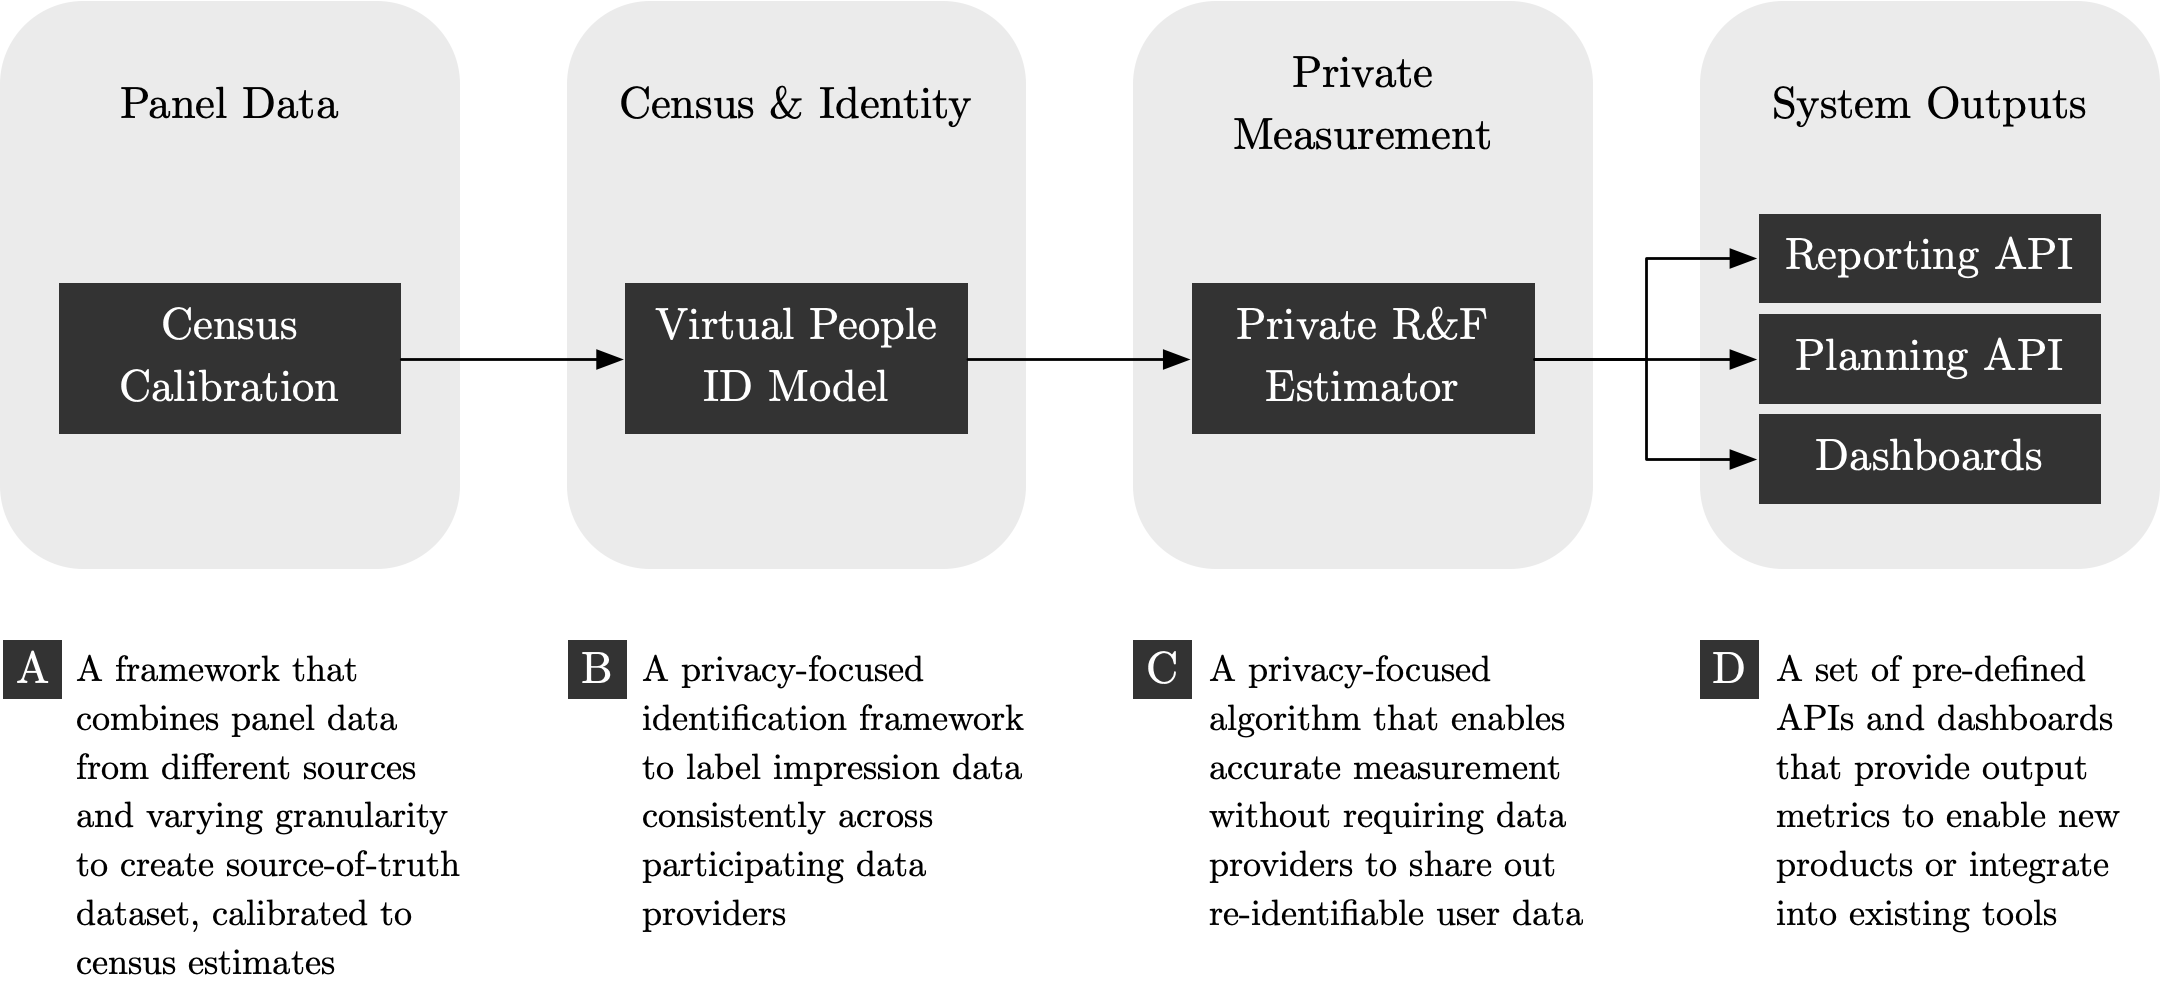
\includegraphics[width=\textwidth]{image1.png}
\centering
\end{figure}
\vspace*{0.5cm}

\subsubsection{1. Panels as source of truth}

In order to capture all relevant media consumption data, data providers will need to contribute census data in a privacy centric way. However, to ensure the system is fair and objective, the technical blueprint must
enable independent verification and transparency. The main mechanism for this is a single-source panel (or multiple separate panels) to act as the arbiter of truth, providing benchmarks for the use and overlap of
media consumption and correcting for bias in census data logs.

The single-source panel will be used to calibrate and adjust census data collected directly from data providers where appropriate as well as to provide inputs into reach, frequency and deduplication models \hyperref[ref:3]{[3]}, \hyperref[ref:4]{[4]}. The single-source panel may also be used to measure exposure to media where census data is unavailable. For example, smaller publishers without census data can still be measured by the panel. This will ensure a broad coverage of publishers and reduce barriers to entry for those without census data.

If a single source panel is not available in a local market, other data sources will be required. If separate digital and TV measurement data is available, they could be used in conjunction with relationships measured between digital and TV from countries that have a single source panel, or other data sets or assumptions available in the market.

\paragraph{Panel Requirements}

Panel data must contain the participating data providers' ad exposure event information, associated with user device identifiers, and additional contextual and demographic information that can be useful for developing measurement models.

The panel measurement technology must provide mechanisms to prevent participating data providers from learning the identity of the panelists. Technologies can be used to perform double-blind joins of census log data with panelist sessions. This will protect panelists' privacy, and among other benefits, ensure no data provider can influence panelists inappropriately.

In order to uphold our privacy principles of user control and transparency, panelists must provide verifiable consent for their participating data controller event data to be collected and shared with the panel operator.

Digital and TV media need to be handled somewhat differently (\emph{Note: there is significant local expertise in handling TV census data, which should be relied upon in developing a solution for measuring
TV. The following description is one possible approach to incorporating TV census data into the Census Identification Framework}). For both digital and TV media, census data will be calibrated with the single-source panel. However, TV census data, including Set-Top-Box, Smart TV, and OTT data, could be considered household-level data (depending on the device). This means that it has higher co-viewing rates than other devices. Therefore, this data will have to be converted to individual-level data, using the single-source panel, before applying the Census Identification Framework, as described below. To enable this,
TV census data must be accompanied by the number of people in each household and their associated contextual and demographic information. To the extent that the TV census data is a subset of the full census, viewership will need to be scaled up using the single-source panel and Census Identification Framework. In addition, there are data quality challenges specific to TV census data that will need to be addressed using the single-source panel.

To the extent that multiple panels are available (e.g, a single-source panel and other single-media panels), there are methods for combining these panels in an optimal way for reach and frequency estimation \hyperref[ref:5]{[5]}.

\subsubsection{2. Census Data \& Identity}

\paragraph{Quality Controls}

Each data provider that has the means to collect census level impression data can choose to contribute this data to the system through the Census Identification Framework and Private Reach and Frequency Estimation.

Data providers are responsible for implementing the necessary mechanisms to filter invalid traffic, appropriate quality controls, and auditing mechanisms required by local markets for both content and ad
impressions, including potential impression-level signals such as contextual and demographic information. Some of these requirements will be outlined in the Global Data Input Specification document. The local
body governing should establish an appropriate process for verification and audits of these mechanisms.

\paragraph{Census Identification Framework}

In order to deduplicate reach across data providers and media types, a common method for identifying users is required. An identification framework will allow individual data providers (e.g., publishers and broadcasters) to identify users at a census-level, and make sure this process is consistent across all channels.

There are at least two challenges with this. The first one is designing an identification framework that upholds our privacy principle of non re-identification. The second one is ensuring the quality and coverage
of the existing data.

The technical working group has identified two identification frameworks that address both of these challenges. We propose:

\begin{enumerate}
\def\labelenumi{\arabic{enumi}.}
\tightlist
\item
  Virtual People IDs (VIDs) as a way to solve this problem for reach and frequency immediately \hyperref[ref:6]{[6]};
\item
  A cross-industry effort to explore more advanced methods like the creation of a Secure Universal Measurement ID (SUMID) that could both power metrics for sales lift and multi-touch attribution, and enhance the quality of reach and frequency measurement
\end{enumerate}

We believe these two approaches both help protect against user re-identification and complement each other, however, additional work is required to determine if a SUMID can meet our requirements and principles. The technical working group therefore recommends a future WFA workstream focused on relevant research to develop a SUMID over time. Any VID and SUMID solution will de-link the VIDs and/or SUMIDs from user data to protect against re-identification of users.

\subparagraph{Virtual People IDs (VID)}

Virtual People IDs allow us to generate a common virtual identifier or set of identifiers for every impression, the latter of which is useful for modeling co-viewing. This is done by injecting the statistical information of user activity measured by the Panel into the Data Providers' census data.

The main value of VIDs comes from the fact that:

\begin{itemize}
\tightlist
\item
  Every impression from every Data Provider, including TV and digital,
  is assigned a VID.
\item
  The reach and frequency distribution of VIDs over a particular segment
  of census impressions is a high quality estimator of the true people
  reach and frequency distribution of that segment.
\item
  VIDs can be assigned independently by each Data Provider, using a
  common Panel trained model. No census data needs to be shared between
  Data Providers in order to assign VIDs.
\end{itemize}

It is worth noting that VIDs are statistical in nature, and there is no guarantee that a single person will be assigned the same VID across multiple participants. This means that \emph{in aggregate} VIDs allow
for accurate reach and frequency measurement.5 However, since they do not correspond to real people individually, VIDs can not be used for targeting purposes, nor can they support 1P audiences.

The VID framework implementation can be broken into two phases, described in detail below. Additionally, to ensure that the system upholds our privacy requirements, VIDs need to be combined with methods
that can deduplicate counts of VIDs across Data Providers in a privacy centric way. We discuss these private reach and frequency estimation methods below.

\subparagraph{Secure Universal Measurement IDentity (SUMID)}

Given the current and upcoming changes to how third-party cookies behave on browsers and potential future changes to persistent mobile identifiers, more data providers (both large and small) are relying on
signed-in experiences to establish a direct relationship with their users. This enables data providers to leverage email addresses or other data as common identifiers for the purposes of cross-media measurement.

It should also be possible to add multi-key identifiers to the system, which will improve quality and coverage over just a single identifier such as email. However, for this to be viable, the multi-key identifier
has to be both secure and private, which requires significant technical work and research.

The use of common identifiers for measurement also necessitates industry-wide legal and policy discussions (and consensus) that may take time to develop. On the other hand, leveraging such frameworks will enable more advertiser use cases, such as 1P audiences for reach, sales lift and multi-touch attribution. To that end, the technical working group recommends a future WFA-led workstream to continue development of a privacy centric, industry accepted SUMID.

\subparagraph{Comparison of VID and SUMID}

The VID model is much more than a mechanism for assigning common IDs, as it provides a modeling layer that is necessary to account for TV data, logged-out traffic, co-viewing, and calibration of census data to a
panel. Even once SUMID is implemented, the VID model, or something similar, will still be required.

SUMID alone will not have 100\% coverage of the cross-media input data:

\begin{itemize}
\tightlist
\item
  Logged-out traffic on the web, even where a stable first party cookie
  exists, will not be mappable to a SUMID. These cookies can still be
  used to create VIDs.
\item
  A large fraction of TV devices will not be mappable to a SUMID.
\item
  Opted-out users will not be mappable to a SUMID
\end{itemize}

Moreover, even if SUMIDs were augmented with demographic attributes, an additional layer of modeling would be required to account for device sharing and co-viewing. It is also reasonable to expect that a SUMID with demographic attributes would require the application of techniques similar to those used for VID construction, and would almost certainly include calibration of the demographic assignments to a panel.

We see two ways SUMID can be integrated and complement the R\&F VID solution. One way is with a standalone SUMID integration where we continue to generate VID based estimates but can also generate a new set of SUMID based estimates. In this type of integration we could add an additional layer of post correction to the VID estimates based on the SUMID estimates.

Another more comprehensive approach is where SUMIDs are integrated more directly in the panel used to train VID models, and used as one of the stable identifiers for mapping impressions to VID. This approach will likely lead to higher quality and scalable long term results, but comes with a new set of privacy preserving computation challenges that need to be explored and addressed.

While we believe that a VID-only solution is the best way to get started, we also believe that a SUMID+VID-based system is the best long-term solution. It will provide more accurate VID assignment and enable features like 1P audience measurement that the VID-only system is not capable of. Nonetheless, the features of the VID model, which include demographic correction, support for logged-out users, device
sharing and co-viewing modeling, and TV modeling will play a central role even as we incorporate SUMIDs into the solution.

\begin{longtable}{
|>{\hspace{0pt}}m{0.173\textwidth}
|>{\hspace{0pt}}m{0.322\textwidth}
|>{\hspace{0pt}}m{0.443\textwidth}|
}
\caption{Comparison of VID and SUMID frameworks}\\ 

\hline
\rowcolor[rgb]{0.82,0.82,0.82}
\multicolumn{1}{|>{\centering\hspace{0pt}}m{0.173\textwidth}|}{Considerations} & 
\multicolumn{1}{>{\centering\hspace{0pt}}m{0.322\textwidth}|}{Secure Universal Measurement ID (SUMID)} & 
\multicolumn{1}{>{\centering\arraybackslash\hspace{0pt}}m{0.45\textwidth}|}{Virtual People ID (VID)} 
\endfirsthead 

\hline
Meets WFA Framework Privacy Principles\par{} & TBD. Subject to additional research.\par{} & Yes \\ 

\hline
Produces high quality measurement outputs\par{} & TBD. Subject to additional research.\par{} & Yes, for R/F\par{} \\ 

\hline
Enables key use cases\par{} & R/F (improved when used with VID)\par{}Sales outcomes (lift, MTA)\par{}First Party Audience\par{} & R/F\par{}(Further research necessary to see if it can solve other metrics like MTA by itself).\par{} \\ 

\hline
Scales (i.e. accessible to all types of data providers) & No~\par{}(excludes data providers without 1P relationship with users)\par{} & Yes \\ 

\hline

\rowcolor[rgb]{0.82,0.82,0.82} 
Recommendation:\par{} & 
\multicolumn{2}{>{\hspace{0pt}}m{0.8\textwidth}|}{\textbf{Over time the system should support both VID and SUMID.} In the short term, we recommend using VID to deliver reach and frequency measurement without delay, while we continue the WFA-led workstream to develop SUMID.~ } \\
\hline
\end{longtable}






\subsubsection{3. Private Reach and Frequency Estimation}

Once a common method for identifying users has been established, it becomes possible to count impressions across data providers and to compute deduplicated reach and frequency. Due to its consistent approach to modeling, the Virtual People ID model makes this a simple matter of counting unique VIDs across data providers. To accomplish this, data providers would provide VIDs by campaign and user segment to an independently operated measurement service that can combine and deduplicate VIDs to produce an overall estimate of deduplicated reach and frequency.

The WFA technical working group is \href{https://github.com/world-federation-of-advertisers/cardinality_estimation_evaluation_framework/blob/master/doc/cardinality_and_frequency_estimation_evaluation_framework.md}{currently evaluating several candidate solutions} for securely and privately computing deduplicated reach and frequency in this way. Each of these
solutions ensures that no information beyond the agreed upon outputs of the system is learned by any party and that the presence (or absence) of any single individual's data does not appreciably change the output of the system. In short, regardless of which method is chosen, data providers should feel confident that their data is being used only for the agreed upon calculations, and that the privacy of users will be
maintained.

We are currently in the process of evaluating several candidate solutions according to a comprehensive evaluation framework developed with input from the MRC. The \href{https://github.com/world-federation-of-advertisers/cardinality_estimation_evaluation_framework/blob/master/doc/cardinality_and_frequency_estimation_evaluation_framework.md}{framework} is described in full on our GitHub repository, where the \href{https://github.com/world-federation-of-advertisers/cardinality_estimation_evaluation_framework}{source code} for the framework itself and all of the candidate methods can also be found. Some \href{https://github.com/world-federation-of-advertisers/cardinality_estimation_evaluation_framework/tree/master/results}{preliminary results} are also available.

Once the evaluation is complete, a comprehensive set of results and a detailed report will be made available for review.


\subsubsection{4. System Outputs}
This system is designed to produce standard metrics (i.e.~default reporting), Advertiser-defined metrics and a data API that can be accessed broadly. The API can be made available to multiple
organizations, including advertisers, agencies, research vendors, publishers to support new measurement products and/or existing tools. In addition to the API, local markets may also choose to develop a standard
user interface that supports default metrics and Advertiser-defined metrics for users who cannot leverage the API. A list of output metrics that the API and these default reports produce will be determined at the
local level.

\subsection{Key Technical Roles}

This design will require the support and participation of many industry
stakeholders. We've listed some of the roles and responsibilities below.
These roles are not mutually exclusive - i.e.~a `User Impression Data
Provider' may also be a `Private Estimation Node Operator' as
appropriate. The specific stakeholders selected for each of these roles
should be decided at a local market level. Local markets may also
require additional roles to support specific governance structures.

\subsubsection{User Impression Data Providers}

Participating user impression data providers (both digital publishers and OTT data providers) integrate these data sets with the Panel(s), in coordination with Panel Operators, for the purposes of training VID
models in the Setup Phase, and using those models to label user impression data to produce measurement outputs in the Live Measurement Phase \emph{(Note: detailed explanation of VID models and phases
below).}

\subsubsection{Panel Data Provider(s)}
Licenses or provides the panel data, coordinating with different User Impression Data Providers, and providing the output panelist data to the VID Model Operator for the purposes of training a VID model.


\subsubsection{TV RPD Providers}
Provides RPD TV (STB, smartTV, etc) data to the VID model operator that can be used to enrich TV panel data sets to create more accurate VID models for TV, and more comprehensive TV assets.


\subsubsection{Private Estimation Node Operators}
Private estimation methods require running a decentralized (multi-party compute) system where the security is guaranteed by the decentralized nature of the system. In other words, multiple operators are necessary to run the system in a secure way. Participating User Data Providers must trust at least one of the Private Estimation Node Operators in order to trust the security of the system.

\subsubsection{VID Model Operator}
The VID Model Operator has the responsibility of training and releasing VID models using the Panel and TV data assets. It is responsible for collecting other sources of data and the necessary parameters to train
the model, as well as timely updates to the model to meet the local market requirements.

\subsubsection{Measurement API Service Operator}
The measurement API operator owns the reporting layer on top of the Measurement System, and is responsible for enforcing the necessary access control, as well as additional functionality built on top of the
outputs of the measurement system, including potentially standard reports published to the market participants with the required licenses (also enforced by the Measurement API Service Operator).


\subsection{Design Details}

\subsubsection{System Overview and Lifecycle}
Advertisers require that the cross-media measurement system be always-on and not require a resource-intensive set-up process. While a common campaign taxonomy may still be needed to address this (i.e.~how to name campaigns, creatives, etc., consistently across data providers), the technical design should support always-on, tagless measurement and not place an onerous technical burden on participating data providers.

The system is designed to work in two phases: a set-up phase, and an ongoing measurement phase.
 \pagebreak

\subsubsection{Set-Up Phase}


\begin{figure}
\caption{Overview of measurement system set-up phase}
\vspace*{0.5cm}
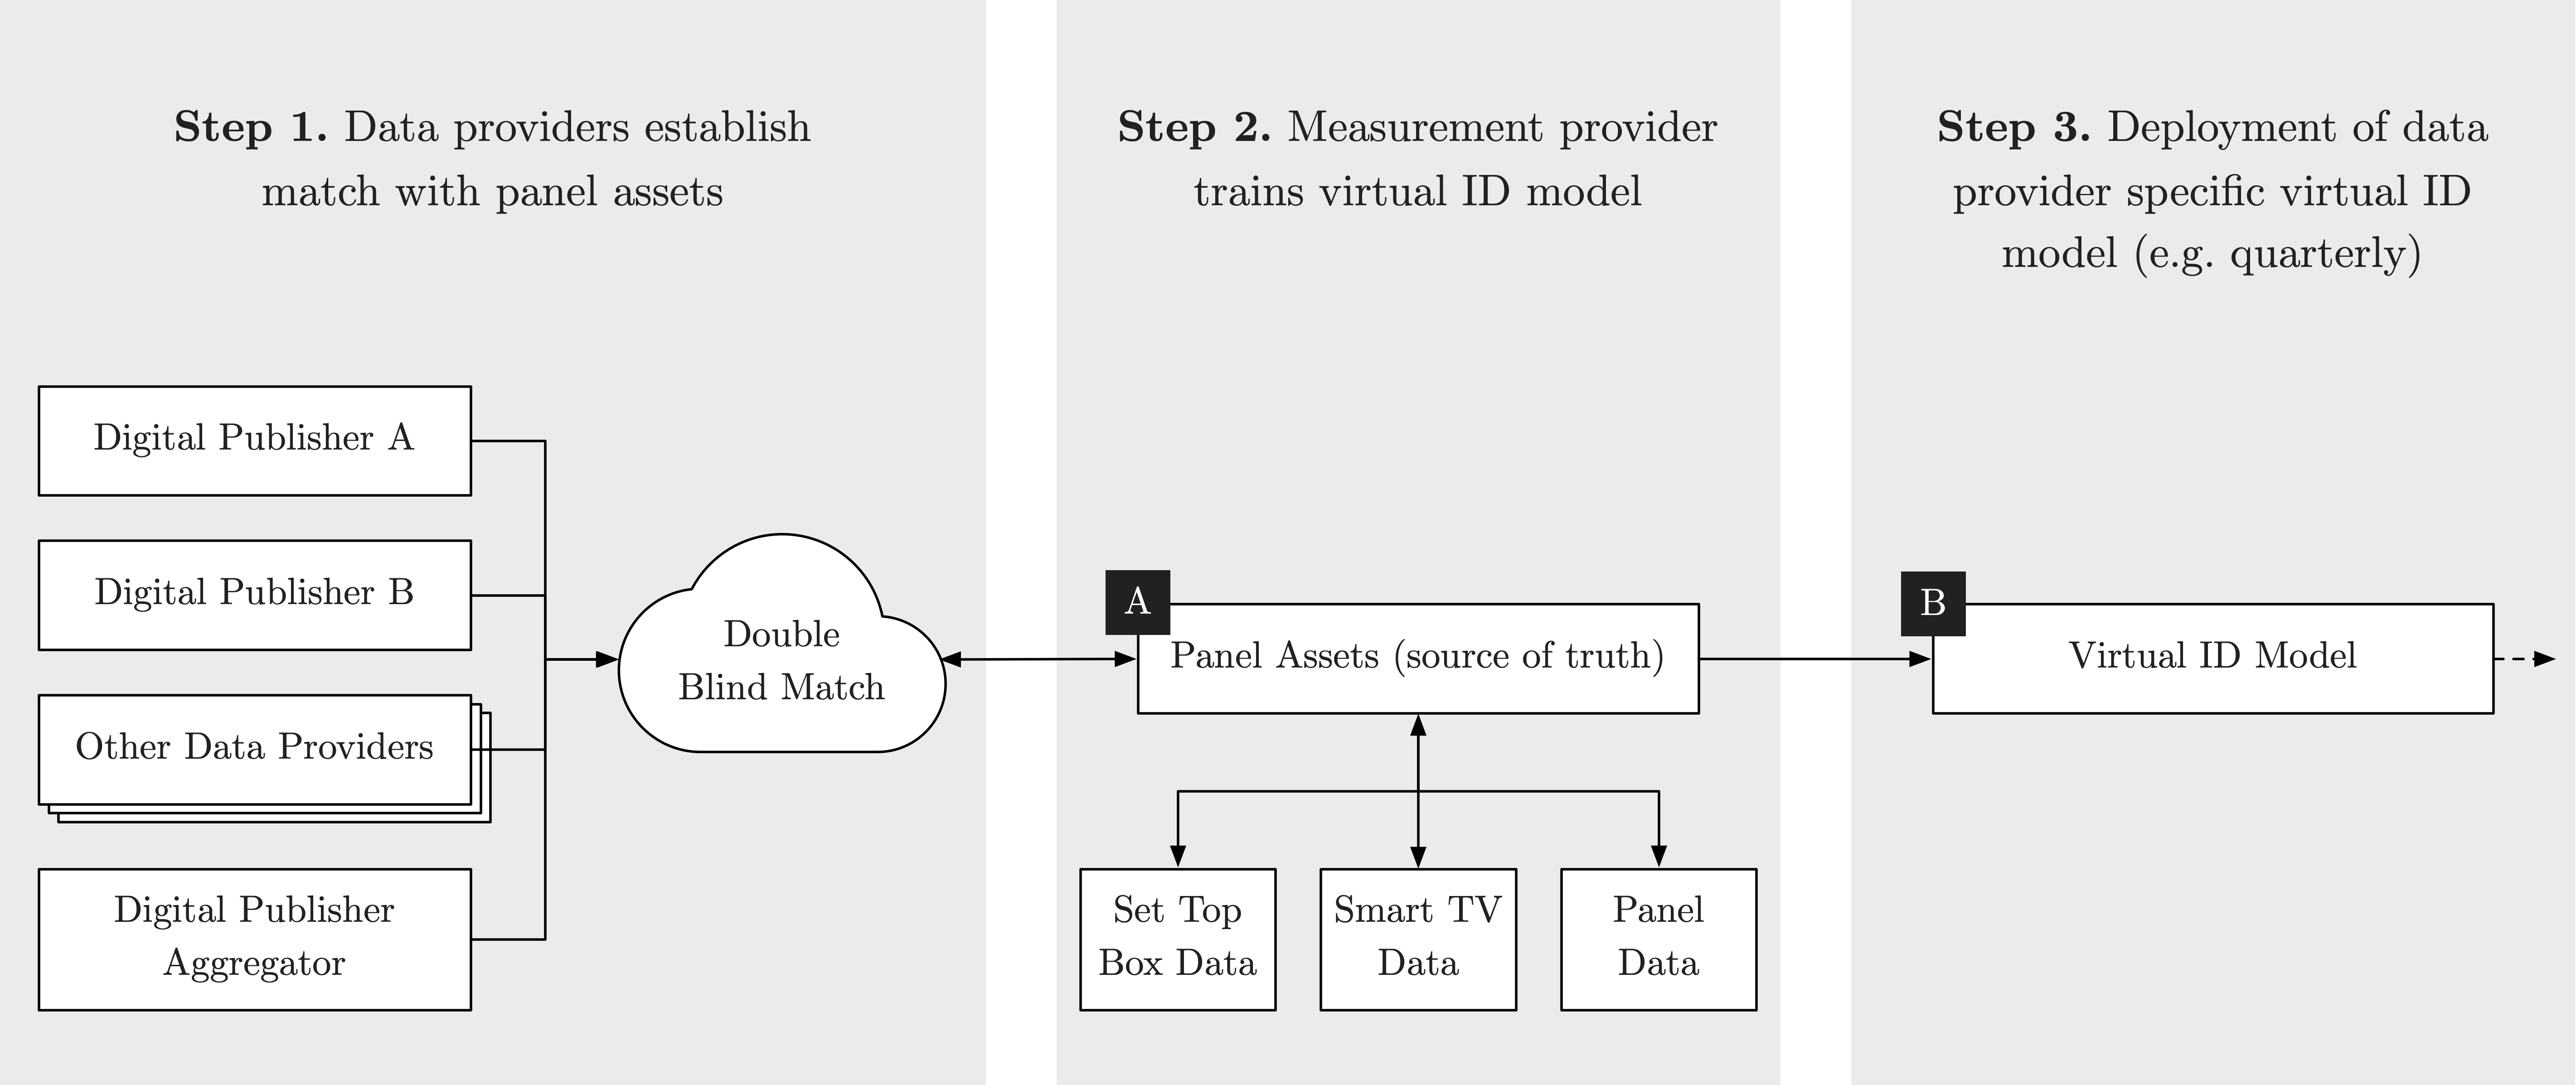
\includegraphics[width=\textwidth]{image2.png}
\centering
\end{figure}
\FloatBarrier
\vspace*{0.5cm}

The main objective of the set up phase is to train a market-specific Virtual People identity model, which will provide the foundation for cross-media deduplication. This set-up process must be completed at the
country/market level and refreshed a few times per year. The specific cadence of updates will depend on a number of factors, including but not limited to the country's rate of population growth and rate of internet
penetration. For example, a developed market with a relatively stable population and higher internet penetration (e.g., US, CA) may only require annual updates. On the other hand, developing countries with
rapid population growth and evolving internet penetration (e.g., IN, ID) may benefit from a quarterly cadence. This should be left up to local governing bodies to decide based on relevant market factors.


\paragraph{Step 1. Data Providers establish match with panel assets}

In the first step of the set up phase, the panel operator and the data participants establish a mechanism to measure ad event data for the participating panelists. This is accomplished through metering technologies as part of the panel, and through an offline double-blind data exchange with data providers, including digital publishers and TV broadcasters with OTT logs. Double-blind data exchanges allow data providers to share consented panelist data without knowing who panelists are, and without revealing sensitive information.

For TV data providers, Set-Top-Box (STB) data, and Smart TV data will be used to establish a match with a Return Path Data (RPD) Panel and provide feature data for the matched panelists.

Taken together this data will enable the collection of the necessary event- and user-level signals required to train the VID model.

\paragraph{Step 2. Measurement Service trains virtual ID model}
After the local measurement service receives all the data for the matched panelists, a VID model will be trained. This model encapsulates the relationship of user activity across demographic groups and data
providers, measured and calibrated by the panel. This step is performed by the VID Operator, using local market insights and benchmarks (e.g., country specific population data), as well as the panel assets, in order to calibrate the output to the target population. For markets where it is desired, multiple VID Models trained by distinct VID Operators can also be supported.


\paragraph{Step 3. Data-provider-specific virtual ID model}
In the last step of the set-up phase, the operator of the measurement service will send the trained data-provider-specific VID model to each participating data provider.



\vspace*{0.5cm}
\subsubsection{Live Campaign Measurement Phase}

\vspace*{0.2cm}
\begin{figure}
\caption{Overview of live campaign measurement phase}
\vspace*{0.5cm}
\vspace*{0.2cm}
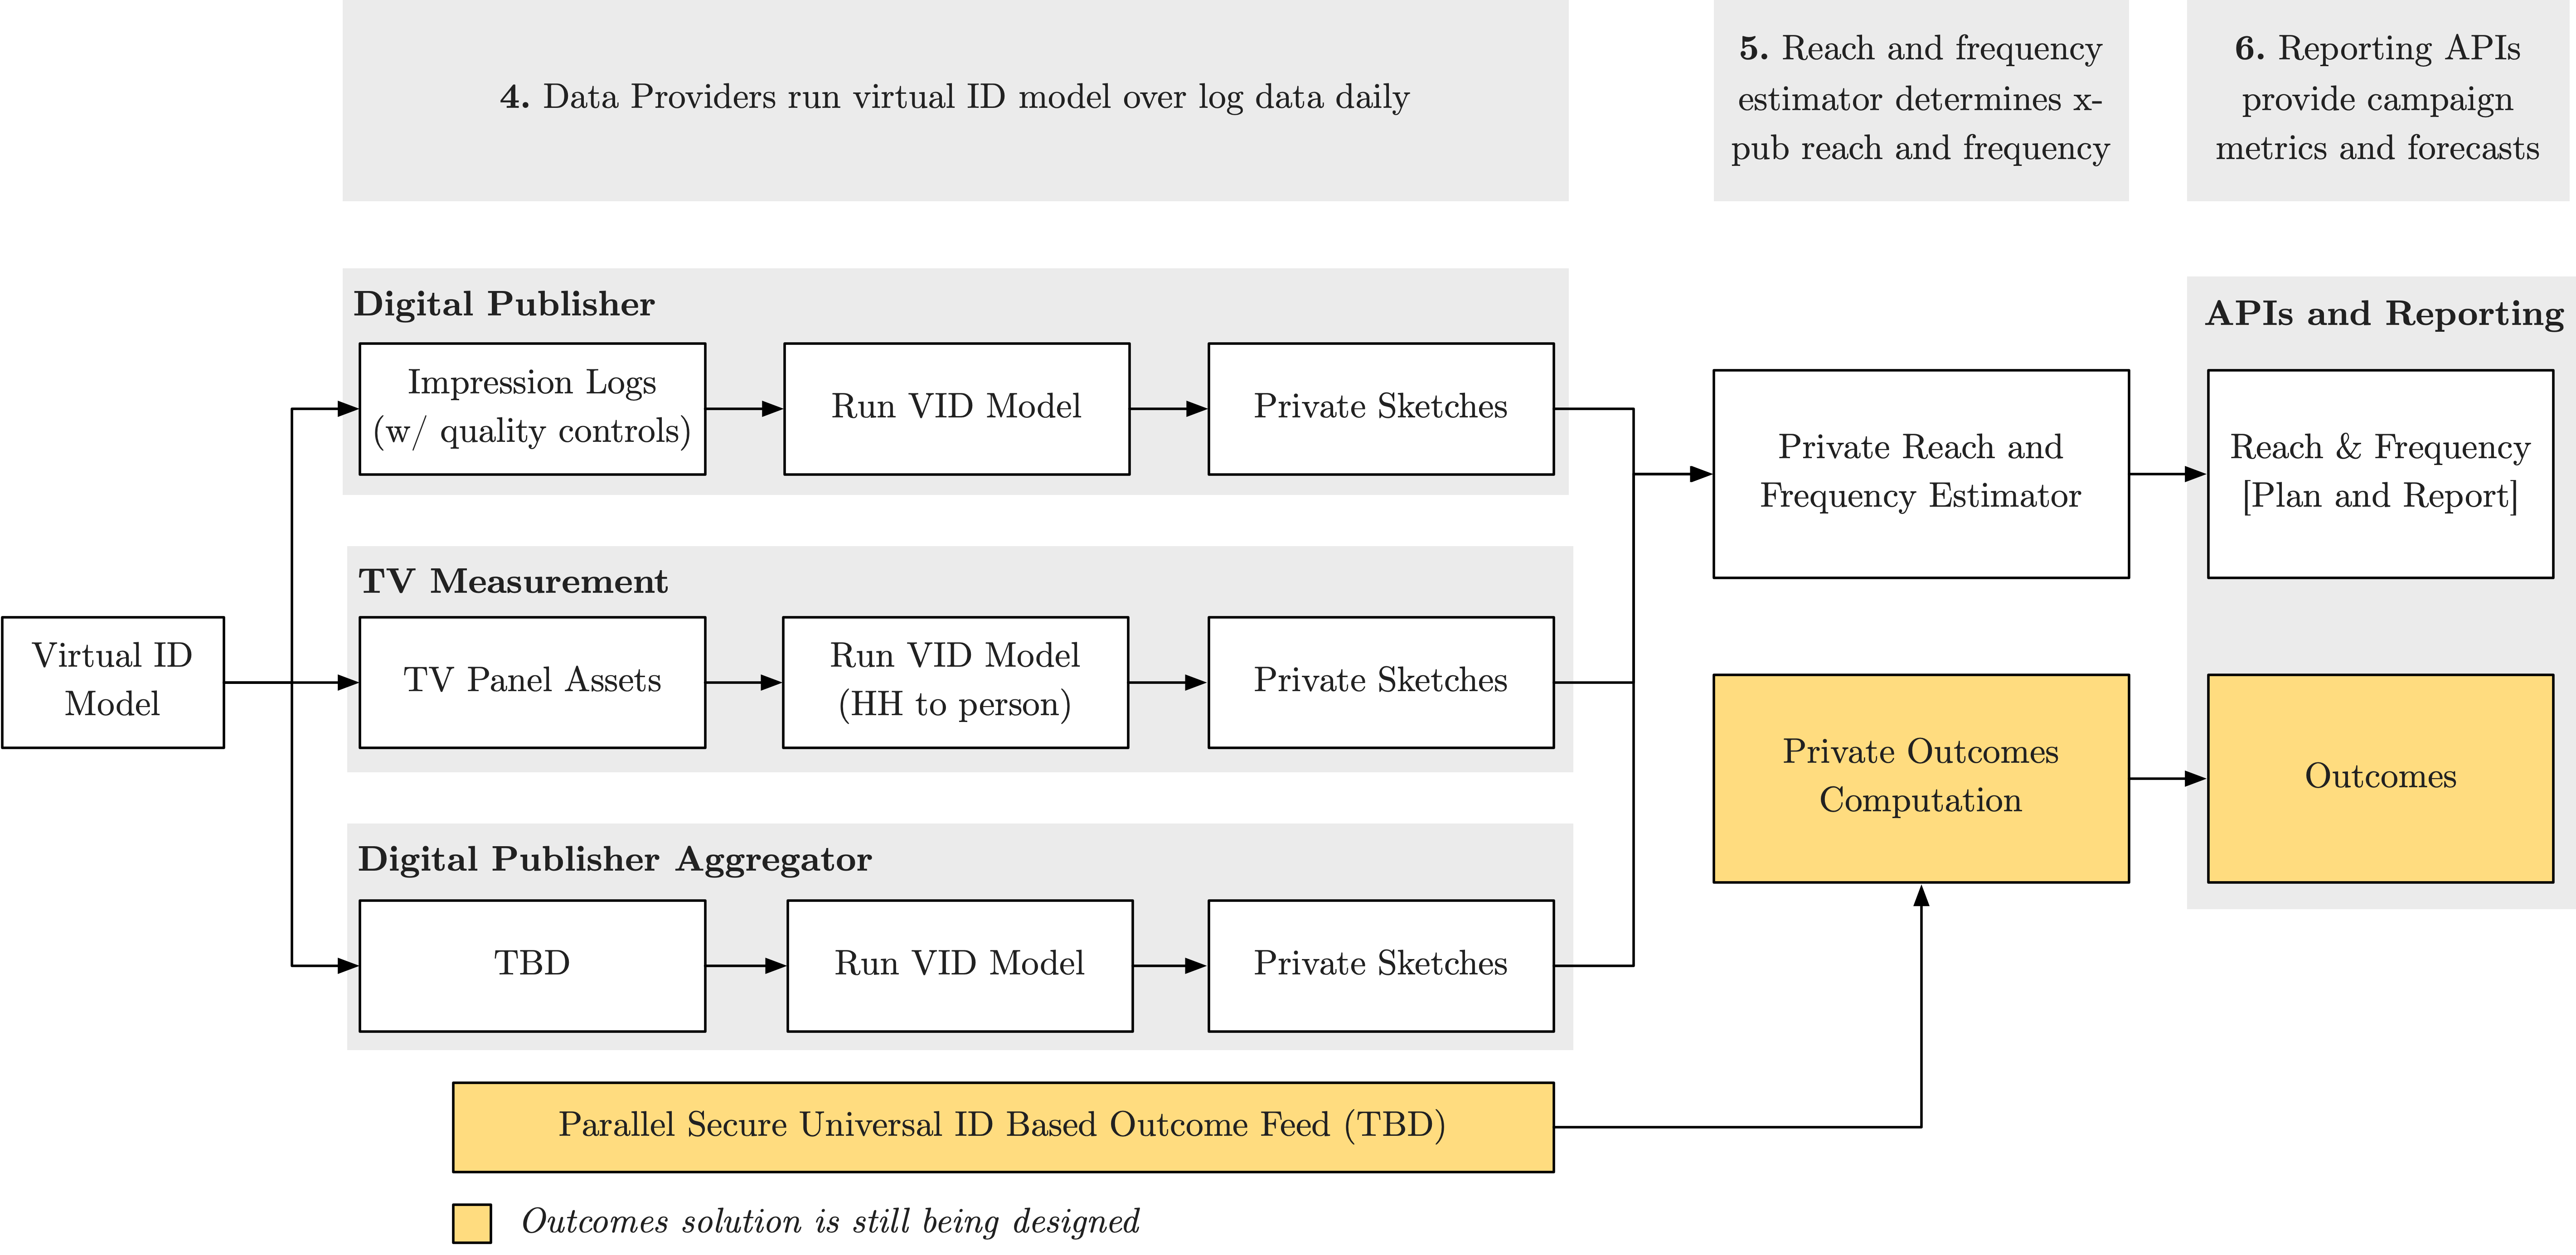
\includegraphics[width=\textwidth]{image3.png}
\centering
\end{figure}
\vspace*{0.5cm}

The second phase of the cross-media measurement is the live campaign measurement phase. This phase happens on a daily basis for the duration of each campaign. In this phase, data providers will label their
campaign impression data with VIDs, and then transform the labelled impression data to private sketches\\
to be processed with the private reach and frequency estimator. This measurement service will then combine the private reach data from multiple data providers and supply standard reach and frequency metrics through an API(s) and/or default reports. Planning APIs will also be provided.


\paragraph{Step 4. Data Providers run Virtual ID model on campaign impression data}

In the live measurement phase, digital and TV data providers will collect campaign impression data on a daily basis. With the data-provider-specific VID model from Phase 1, publishers will be able to assign Virtual IDs and reporting attributes (e.g., age and gender) to the identifiers (e.g., email address, cookie, device ids, etc.) associated with their campaign impression data. Since all the VIDs that different publishers use to label their impression data are drawn from the same virtual population, they enable deduplication across multiple data providers and media in later steps.

Once the raw campaign-level impression data is processed by the VID labeller, each impression will have been assigned a VID and a user segment. Next, the data provider will generate aggregate representations
of this set ofVIDs, possibly one for each combination of campaign and user segment. These aggregate representations are called sketches, which in their raw form are not privacy preserving. Next, each sketch will be transformed into a private sketch in order to help preserve user privacy. This transformation, depending upon the details of the algorithm used to estimate reach and frequency, can entail either the
addition of differentially private noise or encryption. Finally, once the private sketch has been built, the data provider can transmit it to the measurement service where it can be combined with sketches from other data providers.

It is important to recognize that the running of the VID model and the construction of sketches are both performed by data providers within their own computing environments and that raw impression data will never leave their environments.

A turnkey solution for labeling logs and generating sketches that runs on public cloud infrastructure can be provided for data providers that are unable to implement this integration.

\paragraph{Step 5. Reach and frequency estimator determines cross-publisher reach and frequency}

Upon receiving private sketches from multiple data providers, the measurement service will combine the sketches for each campaign and segment and determine the deduplicated reach and frequency across data
providers.

\emph{{[}Additional details will be added to this section once the exact method for computing reach and frequency has been established{]}}


\paragraph{Step 6. Reporting APIs provide campaign metrics}

The next step of the live campaign measurement phase is for the measurement service to provide campaign metrics (reach and frequency) through standard reporting APIs. These services can be accessed by any licensed user subject to data governance and usage rules established by local governing bodies.


\section{Glossary}

\textbf{Census Identification Framework} - A system for applying identifiers to census data in either a deterministic or statistical matter so that accurate measurement can be enabled.

\textbf{Cryptography} - A family of techniques that allows data to be encoded in such a way that only those parties who have the correct key can decode it. Without this key the encoded data is indistinguishable
from random bits. One cryptographic technique, called homomorphic encryption, allows data (e.g.~numbers) to be combined (e.g.~by summing) while encrypted such that the combined encoded data can be decoded while preserving the properties of the function that did the combination (e.g.~the sum).

\textbf{Data Provider} - An entity that provides census data for reach and frequency estimation. This term is used in place of publisher and/or broadcaster and is meant to abstract away the difference between providers of various media types.

\textbf{Differential Privacy} - A privacy framework that provides a mathematical guarantee of whether anything can be learned about any individual whose data may (or may not) have been used as an input to an reach/frequency estimate.1

\textbf{Double Blind Match} - A process whereby multiple entities share data via a cryptographic protocol that allows comparison of data without divulging the actual data itself.

\textbf{Measurement Phase} - The part of the system that processes publisher census and produces reach and frequency measurements.

\textbf{Re-identification} - The process by which seemingly anonymous data is joined with other data sources in order to reveal the identities of individuals in the first ``anonymized'' data set. For \href{https://arstechnica.com/tech-policy/2014/06/poorly-anonymized-logs-reveal-nyc-cab-drivers-detailed-whereabouts/}{example}, poorly anonymized New York City taxi cab records revealed the comings
and goings of the city's taxi cab drivers over the course of about 173 million trips.

\textbf{Secure Universal Measurement ID (SUMID)} - A deterministic cross media user identifier. The SUMID system uses multiple common user identifiers to securely and privately match users across different data
providers.

\textbf{Setup Phase} - The part of the system that is concerned with collecting panelist data and training a Virtual ID model for deployment.

\textbf{Virtual People ID (VID)} - An identifier that is assigned to census data based on a panel-calibrated model. The VID model also assigns segment information to the census data.


\section{References}

\begin{enumerate}[label={[\arabic*]}]

% \def\labelenumi{\arabic{enumi}.}
\tightlist
\item
  \href{https://georgetownlawtechreview.org/wp-content/uploads/2017/04/Lubarsky-1-GEO.-L.-TECH.-REV.-202.pdf}{Re-identification of ``Anonymized Data''} (2017) \label{ref:1}
\item
  \href{https://www.cis.upenn.edu/~aaroth/Papers/privacybook.pdf}{The Algorithmic Foundations of Differential Privacy} (2014) \label{ref:2}
\item
  \href{https://research.google/pubs/pub41089/}{A Method for Measuring Online Audiences} (2013) \label{ref:3}
\item
  \href{https://research.google/pubs/pub45353/}{Measuring Cross-Device Online Audiences} (2016) \label{ref:4}
\item
  \href{https://research.google/pubs/pub42246/}{Data enrichment for incremental reach estimation} (2014) \label{ref:5}
\item
  \href{https://research.google/pubs/pub48387/}{Virtual People: Actionable Reach Modeling} (2019) \label{ref:6}
\end{enumerate}



\end{document}
